%============================================================================%
%
%	DOCUMENT DEFINITION
%
%============================================================================%

%we use article class because we want to fully customize the page and don't use a cv template
\documentclass[10pt,a4paper]{article}

%----------------------------------------------------------------------------------------
%	ENCODING
%----------------------------------------------------------------------------------------

% we use utf8 since we want to build from any machine
\usepackage[utf8]{inputenc}

%----------------------------------------------------------------------------------------
%	LOGIC
%----------------------------------------------------------------------------------------

% provides \isempty test
\usepackage{xstring, xifthen}

%----------------------------------------------------------------------------------------
%	FONT BASICS
%----------------------------------------------------------------------------------------

% some tex-live fonts - choose your own

%\usepackage[defaultsans]{droidsans}
%\usepackage[default]{comfortaa}
%\usepackage{cmbright}
\usepackage[default]{raleway}
%\usepackage{fetamont}
%\usepackage[default]{gillius}
%\usepackage[light,math]{iwona}
%\usepackage[thin]{roboto}

% set font default
\renewcommand*\familydefault{\sfdefault}
\usepackage[T1]{fontenc}

% more font size definitions
% \usepackage{moresize}
 \usepackage{moresize}

%----------------------------------------------------------------------------------------
%	FONT AWESOME ICONS
%----------------------------------------------------------------------------------------

% include the fontawesome icon set
\usepackage{fontawesome}

% use to vertically center content
% credits to: http://tex.stackexchange.com/questions/7219/how-to-vertically-center-two-images-next-to-each-other
\newcommand{\vcenteredinclude}[1]{\begingroup
\setbox0=\hbox{\includegraphics{#1}}%
\parbox{\wd0}{\box0}\endgroup}

% use to vertically center content
% credits to: http://tex.stackexchange.com/questions/7219/how-to-vertically-center-two-images-next-to-each-other
\newcommand*{\vcenteredhbox}[1]{\begingroup
\setbox0=\hbox{#1}\parbox{\wd0}{\box0}\endgroup}

% icon shortcut
\newcommand{\icon}[3] {
	\makebox(#2, #2){\textcolor{maincol}{\csname fa#1\endcsname}}
}

% icon with text shortcut
\newcommand{\icontext}[4]{
	\vcenteredhbox{\icon{#1}{#2}{#3}}  \hspace{2pt}  \parbox{0.9\mpwidth}{\textcolor{#4}{#3}}
}

% icon with website url
\newcommand{\iconhref}[5]{
    \vcenteredhbox{\icon{#1}{#2}{#5}}  \hspace{2pt} \href{#4}{\textcolor{#5}{#3}}
}

% icon with email link
\newcommand{\iconemail}[5]{
    \vcenteredhbox{\icon{#1}{#2}{#5}}  \hspace{2pt} \href{mailto:#4}{\textcolor{#5}{#3}}
}

%----------------------------------------------------------------------------------------
%	PAGE LAYOUT  DEFINITIONS
%----------------------------------------------------------------------------------------

% page outer frames (debug-only)
% \usepackage{showframe}

% we use paracol to display breakable two columns
\usepackage{paracol}

% define page styles using geometry
\usepackage[a4paper]{geometry}

% remove all possible margins
\geometry{top=1cm, bottom=1cm, left=1cm, right=1cm}

\usepackage{fancyhdr}
\pagestyle{empty}

% space between header and content
% \setlength{\headheight}{0pt}

% indentation is zero
\setlength{\parindent}{0mm}

%----------------------------------------------------------------------------------------
%	TABLE /ARRAY DEFINITIONS
%----------------------------------------------------------------------------------------

% extended aligning of tabular cells
\usepackage{array}

% custom column right-align with fixed width
% use like p{size} but via x{size}
\newcolumntype{x}[1]{%
>{\raggedleft\hspace{0pt}}p{#1}}%


%----------------------------------------------------------------------------------------
%	GRAPHICS DEFINITIONS
%----------------------------------------------------------------------------------------

%for header image
\usepackage{graphicx}

% use this for floating figures
% \usepackage{wrapfig}
% \usepackage{float}
% \floatstyle{boxed}
% \restylefloat{figure}

%for drawing graphics
\usepackage{tikz}
\usetikzlibrary{shapes, backgrounds,mindmap, trees}

%----------------------------------------------------------------------------------------
%	Color DEFINITIONS
%----------------------------------------------------------------------------------------
\usepackage{transparent}
\usepackage{color}

% primary color
\definecolor{maincol}{RGB}{ 225, 0, 0 }

% accent color, secondary
% \definecolor{accentcol}{RGB}{ 250, 150, 10 }

% dark color
\definecolor{darkcol}{RGB}{ 70, 70, 70 }

% light color
\definecolor{lightcol}{RGB}{245,245,245}


% Package for links, must be the last package used
\usepackage[hidelinks]{hyperref}

% returns minipage width minus two times \fboxsep
% to keep padding included in width calculations
% can also be used for other boxes / environments
\newcommand{\mpwidth}{\linewidth-\fboxsep-\fboxsep}



%============================================================================%
%
%	CV COMMANDS
%
%============================================================================%

%----------------------------------------------------------------------------------------
%	 CV LIST
%----------------------------------------------------------------------------------------

% renders a standard latex list but abstracts away the environment definition (begin/end)
\newcommand{\cvlist}[1] {
	\begin{itemize}{#1}\end{itemize}
}

%----------------------------------------------------------------------------------------
%	 CV TEXT
%----------------------------------------------------------------------------------------

% base class to wrap any text based stuff here. Renders like a paragraph.
% Allows complex commands to be passed, too.
% param 1: *any
\newcommand{\cvtext}[1] {
	\begin{tabular*}{1\mpwidth}{p{0.98\mpwidth}}
		\parbox{1\mpwidth}{#1}
	\end{tabular*}
}

%----------------------------------------------------------------------------------------
%	CV SECTION
%----------------------------------------------------------------------------------------

% Renders a a CV section headline with a nice underline in main color.
% param 1: section title
\newcommand{\cvsection}[1] {
	\vspace{14pt}
	\cvtext{
		\textbf{\LARGE{\textcolor{darkcol}{\uppercase{#1}}}}\\[-4pt]
		\textcolor{maincol}{ \rule{0.1\textwidth}{2pt} } \\
	}
}

%----------------------------------------------------------------------------------------
%	META SKILL
%----------------------------------------------------------------------------------------

% Renders a progress-bar to indicate a certain skill in percent.
% param 1: name of the skill / tech / etc.
% param 2: level (for example in years)
% param 3: percent, values range from 0 to 1
\newcommand{\cvskill}[3] {
	\begin{tabular*}{1\mpwidth}{p{0.72\mpwidth}  r}
 		\textcolor{black}{\textbf{#1}} & \textcolor{maincol}{#2}\\
	\end{tabular*}%

	\hspace{4pt}
	\begin{tikzpicture}[scale=1,rounded corners=2pt,very thin]
		\fill [lightcol] (0,0) rectangle (1\mpwidth, 0.15);
		\fill [maincol] (0,0) rectangle (#3\mpwidth, 0.15);
  	\end{tikzpicture}%
}


%----------------------------------------------------------------------------------------
%	 CV EVENT
%----------------------------------------------------------------------------------------

% Renders a table and a paragraph (cvtext) wrapped in a parbox (to ensure minimum content
% is glued together when a pagebreak appears).
% Additional Information can be passed in text or list form (or other environments).
% the work you did
% param 1: time-frame i.e. Sep 14 - Jan 15 etc.
% param 2:	 event name (job position etc.)
% param 3: Customer, Employer, Industry
% param 4: Short description
% param 5: work done (optional)
% param 6: technologies include (optional)
% param 7: achievements (optional)
\newcommand{\cvevent}[7] {

	% we wrap this part in a parbox, so title and description are not separated on a pagebreak
	% if you need more control on page breaks, remove the parbox
	\parbox{\mpwidth}{
		\begin{tabular*}{1\mpwidth}{p{0.72\mpwidth}  r}
	 		\textcolor{black}{\textbf{#2}} & \colorbox{maincol}{\makebox[0.25\mpwidth]{\textcolor{white}{#1}}} \\
			\textcolor{maincol}{\textbf{#3}} & \\
		\end{tabular*}\\[8pt]

		\ifthenelse{\isempty{#4}}{}{
			\cvtext{#4}\\
		}
	}

	\ifthenelse{\isempty{#5}}{}{
		\vspace{9pt}
		{#5}
	}

	\ifthenelse{\isempty{#6}}{}{
		\vspace{9pt}
		\cvtext{\textbf{Technologies include:}}\\
		{#6}
	}

	\ifthenelse{\isempty{#7}}{}{
		\vspace{9pt}
		\cvtext{\textbf{Memorable achievements include:}}\\
		{#7}
	}
	\vspace{14pt}
}

%----------------------------------------------------------------------------------------
%	 CV META EVENT
%----------------------------------------------------------------------------------------

% Renders a CV event on the sidebar
% param 1: title
% param 2: subtitle (optional)
% param 3: customer, employer, etc,. (optional)
% param 4: info text (optional)
\newcommand{\cvmetaevent}[4] {
	\textcolor{maincol} {\cvtext{\textbf{\begin{flushleft}#1\end{flushleft}}}}

	\ifthenelse{\isempty{#2}}{}{
	\textcolor{darkcol} {\cvtext{\textbf{#2}} }
	}

	\ifthenelse{\isempty{#3}}{}{
		\cvtext{{ \textcolor{darkcol} {#3} }}\\
	}

	\cvtext{#4}\\[14pt]
}

%---------------------------------------------------------------------------------------
%	QR CODE
%----------------------------------------------------------------------------------------

% Renders a qrcode image (centered, relative to the parentwidth)
% param 1: percent width, from 0 to 1
\newcommand{\cvqrcode}[1] {
	\begin{center}
		
\includegraphics[width={#1}\mpwidth]{image/qrcode.png}
	\end{center}
}


%============================================================================%
%
%
%
%	DOCUMENT CONTENT
%
%
%
%============================================================================%
\begin{document}
\columnratio{0.31}
\setlength{\columnsep}{2.2em}
\setlength{\columnseprule}{4pt}
\colseprulecolor{lightcol}
\begin{paracol}{2}
\begin{leftcolumn}

	%---------------------------------------------------------------------------------------
%	META IMAGE
%----------------------------------------------------------------------------------------
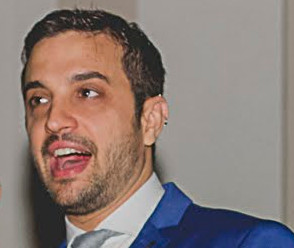
\includegraphics[width=\linewidth]{image/faceLeft.jpg}	%trimming relative to image size

	%---------------------------------------------------------------------------------------
%	META SKILLS
%----------------------------------------------------------------------------------------
\cvsection{SKILLS}

\cvskill{Project Management} {} {1} \\[-2pt]

\cvskill{Team Player} {} {1} \\[-2pt]

\cvskill{Problem-solving} {} {1} \\[-2pt]

\cvskill{Automation/ Mechatronics} {} {1} \\[-2pt]

\cvskill{Open Source Tools} {} {1} \\[-2pt]

\vfill\null
\cvskill{Portuguese} {Native} {1} \\[-2pt]
\cvskill{English} {} {0.8} \\[-2pt]
\cvskill{Spanish} {} {0.7} \\[-2pt]
\vfill\null
	\cvsection{CONTACT}

\icontext{MapMarker}{12}{23-25 Dumaresq Street\\unit 1, Gordon - NSW}{black}\\[6pt]
\icontext{MobilePhone}{12}{+61 423 014 798}{black}\\[6pt]
\iconemail{Envelope}{12}{fesnavarro@protonmail.com}{fesnavarro@protonmail.com}{black}\\[6pt]
\iconhref {Linkedin}{12}{felipe-navarro-7a45515a}{https://www.linkedin.com/in/felipe-navarro-7a45515a}{black}\\[6pt]
\iconhref {Github}{12}{fesnavarro/eCoatKtl}{https://github.com/fesnavarro/eCoatKtl}{black}\\[6pt]
\vfill\null

	\cvqrcode{0.7}

	%---------------------------------------------------------------------------------------
%	QUALIFICATIONS
%----------------------------------------------------------------------------------------
\newpage
\cvsection{ACADEMIC \\ QUALIFICATIONS}

\cvmetaevent
{1999 - 2001}
{Technology in industrial mechatronics}
{Senai "Armando Arruda Pereira"}
{Financially supported by Jica (Japan International Cooperation Agency), the course had all the necessary technology to teach about elements of industrial automation.

	Robots, PLC, controllers, CNC, AGV, RGV, were all equipment available in the school.}

\cvmetaevent
{1996 - 1998}
{General mechanics and machining}
{Senai "Carlos Pasquale"}
{2,5 years +5200 hours course. Full-time course that I started when I was 14 years old.

	The focus of the course was the professional and behavioural training of young people adapting them to the industrial culture of the time.

	All aspects were supervised by the teachers and the course did not include elementary education, which should be done in parallel, requiring an effort common to the adult life of involvement with full-time work and night study.
	The course included industrial technical design, lathes, welding, milling, CNC modelling, metrology.}

\vfill\null

	\cvqrcode{0.7}

	%---------------------------------------------------------------------------------------
%	INTERESTS
%----------------------------------------------------------------------------------------
\newpage
\cvsection{INTERESTS}

\cvmetaevent
{PARAQUEDISMO - Voo livre}
{}
{}
{Paraquedista desde 2009, Eu sou apaixonado pelo esporte, tendo performado saltos e treinamento em tunel de vento em diversas localidades como Russia, Australia, Irlanda, Uruguai, Espanha e Itália.}

\iconhref {Youtube}{12}{FreeFly - Empuriabrava}
{https://www.youtube.com/watch?v=9OdC-JeWI88}{black}\\[6pt]
\iconhref {Youtube}{12}{Windtunnel - Moscow}
{https://www.youtube.com/watch?v=a9Q3ulO_LHU}{black}\\[6pt]
\iconhref {Youtube}{12}{Balloon - São Paulo}
{https://www.youtube.com/watch?v=Wqjl9-4sh5s}{black}\\[6pt]

\cvmetaevent
{OPEN SOURCE - Pesquisador insaciável}
{}
{}
{ Sempre fui envolvido com sistemas de informacão, mas desde 2014 eu decidi me voltar para os sistemas Unix e me tornei absolutamente fã de projetos opensource, desde então eu imergi e me mantive atento a todos os tipos de repositories variados. Sempre que possivel, eu uso meu tempo livre para testar scripts e subir novas infraestruturas que me parecem promissoras. Eu passo tanto tempo olhando através de terminais (bash, sh, zsh), quando obrigado a usar o VSCODE, eu ainda preciso do modo VIM, uso modo VIM pra tudo, mesmo utilizando meu navegador }

\vfill

	\mbox{} % hotfix to place qrcode on the bottom when there are not other elements
	\cvqrcode{0.7}

\end{leftcolumn}
\begin{rightcolumn}
%---------------------------------------------------------------------------------------
%	TITLE  HEADER
%----------------------------------------------------------------------------------------
\fcolorbox{white}{darkcol}{\begin{minipage}[c][3.5cm][c]{1\mpwidth}
	\begin {center}
	\HUGE{ \textbf{ \textcolor{white}{ \uppercase{ FELIPE NAVARRO } } } } \\[-24pt]
	\textcolor{white}{ \rule{0.1\textwidth}{1.25pt} } \\[4pt]
	\large{ \textcolor{white} {Project Manager/ Software Architect} }
	\end {center}
	\end{minipage}} \\[14pt]
\vspace{-12pt}

%---------------------------------------------------------------------------------------
%	PROFILE
%----------------------------------------------------------------------------------------
\vfill\null
\cvsection{PROFILE}

\cvtext{I'm 38, Brazilian, no kids and project manager with strong knowledge
skills and a passion for industrial automation.\\

	Specialised both in automation and in custom application development,
	experienced with large projects and heterogeneous infrastructures. The
	link between development and operations.\\

	Customer-oriented and structured method of working, focused on quality and
	maintainability. Highly motivated to work in a team, both comfortable in
	big companies as in small teams.\\

}

\iconhref {Youtube}{12}{youtube.com/watch?v=Wqjl9-4sh5s}
{https://www.youtube.com/watch?v=Wqjl9-4sh5s}{black}\\[6pt]
%---------------------------------------------------------------------------------------
%	WORK EXPERIENCE
%----------------------------------------------------------------------------------------

\cvsection{WORK EXPERIENCE}

\cvevent
{Fev 16  - Jan 20}
{Project Manager/ DevOps enginneer}
{Research and Development/ Industrial Automation}
{[EIA-ECOD3] - Responsible for defining and managing a software
development team to integrate industrial automation with information
technology using Open Source tools}
{\cvlist{
		\item Deployment and full integration of the company's ERP,
		including all internal and external processes
		\item Deploy and integration of several systems applications
		using AWS, Linode, Google Cloud and others
		for customers such as EPLAN, General Motors, Ross Controls
		\item Management and development of several trade-up in production lines in partnership with
		Rockwell Automation and Edge group
	}}
{\cvlist {
		\item GIT (on GitLab) for all projects, Ansible + Docker for 1-click deployments
		\item Frameworks based on python and javascript like Django,
		Flask, Odoo OEE (WebSockets, REST), QML (QT), React (Typescript,
		GraphQl, Redux)
		\item PostgreSQL, MongoDB
		\item Several open Source tools and projects like Zabbix, Axterisk,
		Matrix (on Riot), Webdav, Bareos, Traefik, Pfsense
	}}
{\cvlist{
		\item Automation from scratch of a painting line with KTL technology
		at Randon Implementos (Caxias do Sul), automation included elements such as Elipse (SCADA)
		superviser system, 4 HMI, local reading in OPCUA by a python client, storage and exposure by https
		for consumption in infrastructure using Grafana in the exhibition
		\item Using an ESP32 (with more internal resources than an Arduino) for local collection
		and transmission, in addition to a RapsberryPI as a consumer gateway for the external
		server API. The integration of the Welding Maintenance Team (General Welding Maintenance - SCS)
		to the ERP Odoo system was resolved in the process, including integrations such as point
		control and automated QRCode reading of the equipment with the ERP
	}}

\cvevent
{Jan 08 - Fev 16}
{Project Manager / Sofware Enginneer}
{Industrial Automation}
{[EIA-SANMARTIN-GOC] - Working for smaller companies I was responsible for
development and administration at the various levels of these companies
whose main customers were large industries}
{\cvlist{
		\item Technical team management with decision and selection of professionals to compose a
		development and installation team
		\item Support and direct development of commercial proposals,
		training and presentations
	}}
{\cvlist {
		\item Barcode position, encoders, Wifi Radios and bluetooth
		\item Working with PMI methodologies, check lists and quality
		procedures
	}}
{\cvlist{
		\item All idealization of the control architecture, development of
		electrical projects and infrastructure in addition to the
		application of general control of the final chassis assembly line at
		Randon Implementos (Caxias do Sul). The project was mentioned in
		international articles as being a pioneer in applying several technologies
		together
		\item I coordinated a massive migration from General Motors (SCS) to General Motors (SJC) plants
		in partnership with Tyssen Krupp, in this project I even defined the
		electrical shutdowns and executed the new start-up in the new plant, the
		project was perfect and almost no application changes were necessary,
		except for integrations between the robotic cells and the local network
		\item In response to a call from Eisemman for automation at MAN (Resende),
		I alone made all the necessary changes for the operation of the Carese
		painting line, with more than 200 conveyors, elevators, transfer tables and
		other elements
		\item In partnership with the company LAN (China) I was able to meet the
		needs in the start-up of the final assembly line at Nissan (Resende) with
		excellence, at the beginning of the work there were many Brazilian and
		Chinese programmers interacting with some difficulty in an environment of
		generalized delay. On the third day I had already rewritten the Chinese codes
		for the start of the lines and I took over as the main responsible for the
		start-up directly with the Japanese from Nissan
		\item Development of automation control and start-up application for AMBEV
		factory (Curitiba), it was the first experience with the beverage industry
		and the project included an industrial washer controlled by 8 servants, two
		boxers, accelerator tables and system integrated vision
	}}

\cvevent
{Jan 05 - Dec 07}
{Software Enginneer}
{Industrial Automation}
{[SPI-TECNEL] - Responsible for the direct development of applications and
parameterization of automated lines in addition to official technical assistance}
{\cvlist{
		\item Direct development of complete software applications
		\item Emergency technical assistance to a range of customers such as
		Alergan (pharmacy), Taboca (mining company), Mercedez Bens (final assembly), General Motors (bodyshop), Coral (chemical), Cofap (parts) and others, demand that required maturity and procedures within the best PMI practices
		\item Official representative of Rockwell do Brasil in projects and
		assistance
	}}
{\cvlist {
		\item Various models of PLC (LADDER, Block Instruction, STL), HMI,
		Inverters, Gateways and other components of Rockwell (Logix 5, 500, 5000),
		Siemens (S5, S7, TIA), Mitsubish, Owron, SEW, ATOS, Schneider, Sick,
		Prosoft
		\item Industrial networks and protocols like Modbus (many), Devicenet,
		Ethernet CIP, Profibus, Profinet, Interbus, DH +, OPC and OPCUA
		\item Integration with robots and tools Fanuc, Kuka, Motoman
	}}
{\cvlist{
		\item Automation of a mining line in the Amazon rainforest under social
		isolation for the production of nickel, using several industrial networks
		integrated in the same system as Modbus. All the work done without external
		assistance during 55 days of start up, there was no internet or any external
		communication within the indigenous village
		\item Software design and development at General Motors for the PRISMA
		automation line, 44 robots and 4 integrated contrologix, that was my first big
		project as a software enginneer, the project had a partnership with Daefuku, which provided
		equipment for the aero system and infrastructure for the new RFID system
	}}

\cvevent
{Jan 01 - Jan 05}
{Electrical Designer}
{Industrial Automation}
{[EIA] - I started as an intern and was promoted in the first months.
Responsible for the development of electrical projects}
{\cvlist{
		\item Electrical projects for various factory standards such as General Motors, Volkswagen,
		Mercedez Bens, Cummins, MWM, Bosh, Pirelli and others
		\item Responsible for quality in the manufacture of panels and field
		interconnection
		\item Purchase of material, and financial monitoring of the project to
		anticipate the budget
	}}
{\cvlist {
		\item Autocad, EPLAN 5.20, ISA ERP (deprecrated), Excell in advance with VB scripts
	}}
{\cvlist{
		\item Several projects in partnership with ThyssenKrupp at Mercedez-SBC
		Bens the biggest one was the complete bodyshop of Mercedez Bens, the first
		line in Brazil entirely handled by AGV
	}}

% hotfixes to create fake-space to ensure the whole height is used
\mbox{}
\vfill
\mbox{}
\vfill
\mbox{}
\vfill
\mbox{}
\end{rightcolumn}
\end{paracol}
\end{document}